% \documentclass[UTF8,oneside]{ctexbook}
% \usepackage{pgfplots}
% \usepackage{caption}
% \begin{document}
% 斯坦福教授、Tcl 语言发明者 John Ousterhout 的著作《A Philosophy of Software Design》,自出版以来,好评如潮。按照 IT 图书出版的惯例,如果冠名为“实践”,书中内容关注的是某项技术的细节和技巧;冠名为“艺术”,内容可能是记录一件优秀作品的设计过程和经验;而冠名为“哲学”,则是一些通用的原则和方法论,这些原则方法论串起来,能够形成一个体系。正如”知行合一”、“世界是由原子构成的”、“我思故我在”,这些耳熟能详的句子能够一定程度上代表背后的人物和思想。用一句话概括《A Philosophy of Software Design》,软件设计的核心在于降低复杂性。

\begin{figure}[!h]
% \centering

\makebox[\textwidth][c]{%
    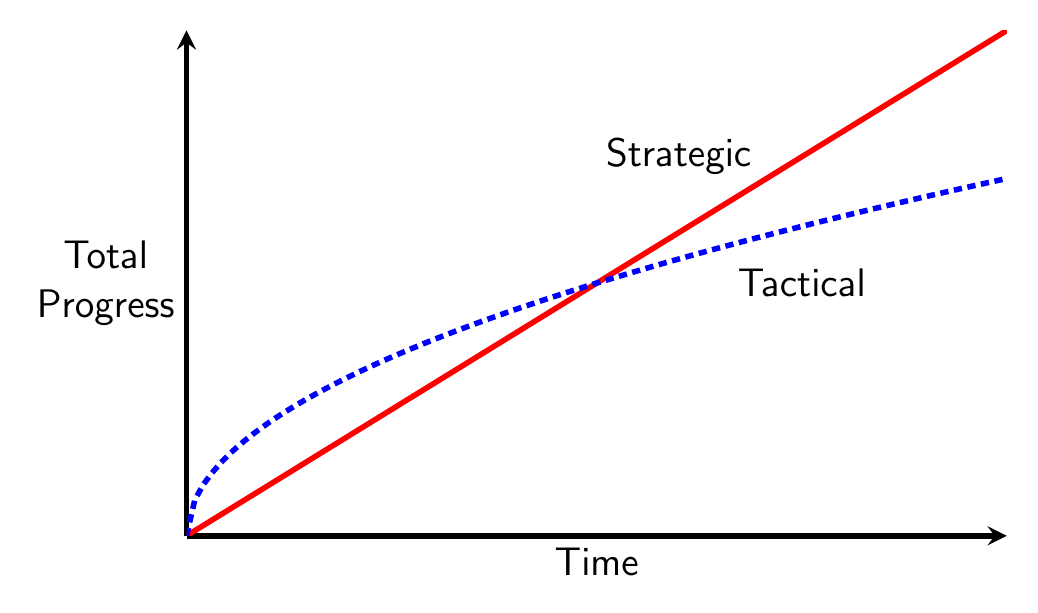
\begin{tikzpicture}[
        font = \sffamily\Large,
        every path/.append style ={line width = 2pt,},
    ]
    \begin{axis}[
        width = 12cm,
        height = 8cm,
        ticks = none,
        axis lines = left,
        xlabel = { Time } ,
        ylabel = { Total\\Progress },
        ylabel style = { rotate = -90, align  = center,},
    ]
    \addplot [domain=0:2,samples=100,color=red ] {x};
    \addplot [
        domain  = 0:2,
        samples = 100,
        color   = blue,
        densely dashed
    ] {x^0.5};
    \node[] at (axis cs: 1.2,1.5) { Strategic};
    \node[] at (axis cs: 1.5,1.0) { Tactical };
    \end{axis}
    \end{tikzpicture}
}%

\caption*{图 3.1}
\label{fig:3-1}
\end{figure}

% \end{document}